% Copyright (C) 2005-2015 Airbus - EDF - IMACS - Phimeca
% Permission is granted to copy, distribute and/or modify this document
% under the terms of the GNU Free Documentation License, Version 1.2
% or any later version published by the Free Software Foundation;
% with no Invariant Sections, no Front-Cover Texts, and no Back-Cover
% Texts.  A copy of the license is included in the section entitled "GNU
% Free Documentation License".
\renewcommand{\filename}{docUC_ThresholdExceedance_FORMExploitation.tex}
\renewcommand{\filetitle}{UC : Run and results exploitation  of a FORM/SORM algorithm : probability estimation, importance factors, reliability indexes, sensitivity factors}

% \HeaderNNIILevel
% \HeaderIILevel
\HeaderIIILevel

\index{Threshold Probability!SORM Breitung, Tvedt, Hohenbichler}
\index{Sensitivity Analysis!FORM probability}
\index{Sensitivity Analysis!Hasofer reliability index}
\index{Graph!FORM/SORM importance factors}
\index{Graph!Hasofer reliability index sensitivity}
\index{Graph Manipulation!View}
\index{Graph Manipulation!Show}



The objective of this Use Case is to launch the analytical algorithm and exploit all the associated results :
\begin{itemize}
\item the design point in both physical and standard space,
\item the probability estimation accoding to the FORM approximation, and the following SORM ones : Tvedt, Hohen-Bichler and Breitung,
\item the Hasofer reliability index and the generalized ones evaluated from the Breitung, Tvedt and Hohen-Bichler approximations,
\item the \emph{classical} importance factors defined as the normalized director factors of the design point in the $\bdU$-space  :
  \begin{equation}\label{def1}
    \alpha_i^2 = \displaystyle \frac{(u_i^{*})^2}{\beta_{HL}^2}
  \end{equation}
  if we note $\vect{u}^*$ the design point in the $\bdU$-space. These importance factors are accessible with the methods \emph{getImportanceFactors(True)} or  \emph{drawImportanceFactors(True)} where the boolean \textit{True} specifies the formula (\ref{def1});
\item the \emph{innovative} importance factors defined in (\ref{def2}) in the elliptical space of the iso-probabilistic transformation, where the marginal distributions are all elliptical, with cumulative distribution function noted $E$, and not yet decorrelated.\\
  In the case where the input distribution of $\vect{X}$ has an elliptical copula $C_E$, then $E$ has the same type as  $C_E$.\\
  In the case where the input distribution of $\vect{X}$ has a copula $C$ which is not elliptical, then  $E=\Phi$ where $\Phi$ is the CDF of the standard normal.\\
  This innovative definition of importance factors has the advantage to be one-to-one between the $X_i$ components and the $Y_i$ ones :
  \begin{equation}\label{def2}
    \alpha_i^2 = \displaystyle \frac{(y_i^{*})^2}{||\vect{y}^{*}||^2}
  \end{equation}
  where
  \begin{eqnarray}
    \boldsymbol{Y}^* =  \left(
    \begin{array}{c}
      E^{-1}\circ F_1(X_1^*) \\
      E^{-1}\circ F_2(X_2^*) \\
      \vdots \\
      E^{-1}\circ F_n(X_n^*)
    \end{array}
    \right).\label{varY10}
  \end{eqnarray}
  with $\vect{X}^*$ the design point in the physical space. If not specified, the importance factors are evaluated from (\ref{def2}).\\
  Note that (\ref{def1}) and (\ref{def2}) match in the case of independent components $X_i$.

\item the sensitivity factors of the Hasofer reliability index and the FORM probability.
\item the coordinates of the mean point in the standard event space :  $\displaystyle \frac{1}{E_1(-\beta)}\int_{\beta}^{\infty} u_1 p_1(u_1)du_1$ where $E_1$ is the spheric univariate distribution of the standard space and $\beta$ the reliability index.
\end{itemize}

Note that it is possible to vizualize the convergence quality of the algorithm, by drawing the history of the  errors defined in the use case \ref{analyticalRes}.


Details on FORM algorithm  may be found in the Reference Guide (\extref{ReferenceGuide}{see files Reference Guide - Step C -- FORM and  - Step Cp -- Importance Factors from FORM-SORM methods}{stepC}).\\


Warning! Check the quality of your gradient and hessian implementations as the SORM approximation relies on an accurate computation of the main curvatures of the limit state function at the design point, which needs an accurate evaluation of both the gradient and the hessian at this point. \\


\requirements{
  \begin{description}
  \item[$\bullet$] the analytical algorithm : {\itshape myAlgoFORM, myAlgoSORM}
  \item[type:] FORM or SORM
  \item[$\bullet$] the limit state function {\itshape model} such as : {\itshape output = model(input)}
  \item[type:] NumericalMathFunction
  \end{description}
}
             {
               \begin{description}
               \item[$\bullet$] SORM Event probabilities (Breitung, HohenBichler and Tvedt approximations)
               \item[type:] NumericalScalar
               \item[$\bullet$] Reliability Index
               \item[type:] NumericalScalar
               \item[$\bullet$] Importance factors
               \item[type:] NumericalPoint
               \item[$\bullet$] Reliability index Sensitivity factors
               \item[type:] AnalyticalSensitivity
               \item[$\bullet$] Mean point in event standard space
               \item[type:] NuemricalPoint
               \item[$\bullet$] graphs
               \item[type:] Graph
               \end{description}
             }

             \textspace\\
             Python  script for this UseCase :

             \inputscript{script_docUC_ThresholdExceedance_FORMExploitation}



             \textspace\\


             The Figure \ref{FORMImportanceFactors}  shows an importance factors pie evaluated from the FORM method, in the beam example described in Eq. (\ref{equatPoutre}), where :
             \begin{itemize}
             \item $E$ follows the Beta($r = 0.94$, $t = 3.19$, $a = 2.78e7$, $b = 4.83e7$) distribution,
             \item $F$ follows the LogNormal($\mu = 3e5$, $\sigma = 9e3$, $\gamma = 1.5e4$)  distribution,
             \item $L$ follows the Uniform($a = 250$, $b=260$) distribution,
             \item $I$ follows the Beta($r = 2.5$, $t = 4.0$, $a = 3.1e2$, $b = 4.5e2$) distribution,
             \item the four components are independant.
             \end{itemize}

             The output is expressed in centimeters.\\
             The event considered is :
             \begin{align*}
               myEvent = \{ output=f(input) \leq -30 \}.
             \end{align*}



             \begin{figure}[H]
               \begin{center}
                 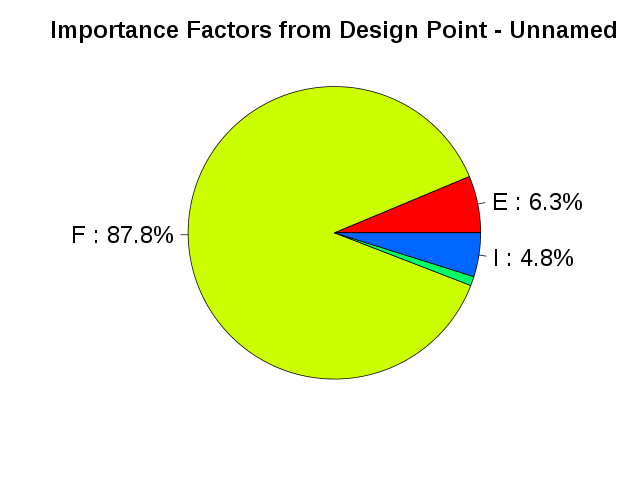
\includegraphics[width=10cm]{Figures/ImportanceFactorsDrawingFORM.png}
               \end{center}
               \caption{Importance factors from the FORM method.}
               \label{FORMImportanceFactors}
             \end{figure}

             \begin{figure}[H]
               \begin{center}
                 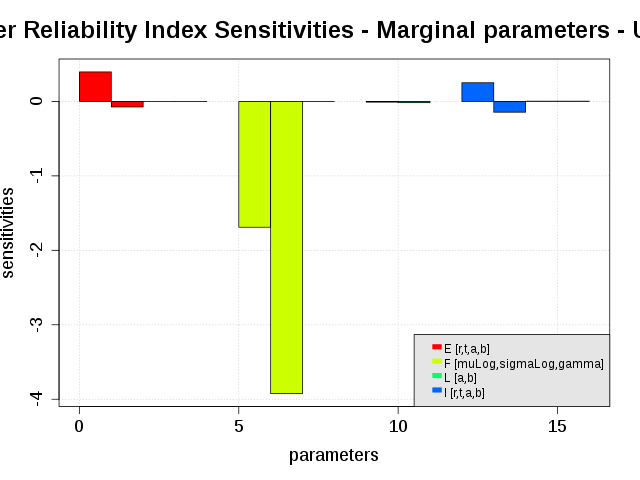
\includegraphics[width=10cm]{Figures/HasoferReliabilityIndexMarginalSensitivityDrawing.png}
               \end{center}
               \caption{Hasofer Reliability Index sensitivities with respect to the marginal parameters.}
               \label{FORMIndexSensitivity}
             \end{figure}

             \begin{figure}[H]
               \begin{center}
                 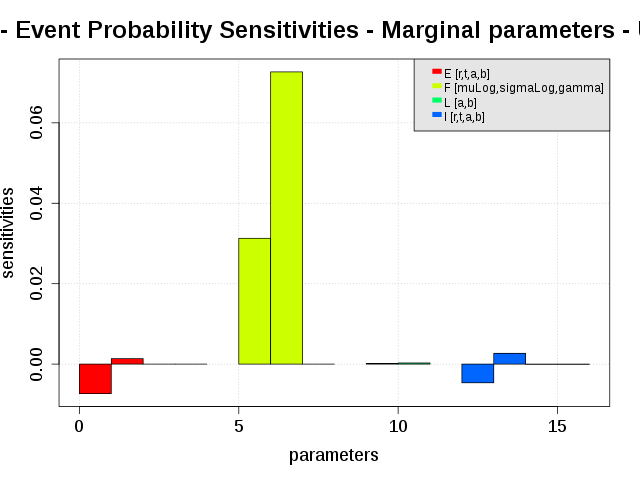
\includegraphics[width=10cm]{Figures/EventProbabilityIndexMarginalSensitivityDrawing.png}
               \end{center}
               \caption{FORM probability sensitivities with respect to the marginal parameters.}
               \label{FORMProbaSensitivity}
             \end{figure}

The Figure \ref{ErrorHist} draws the history of the four errors considered to define the convergence of the algorithm, according to the iteration number.

             \begin{figure}[H]
               \begin{center}
                 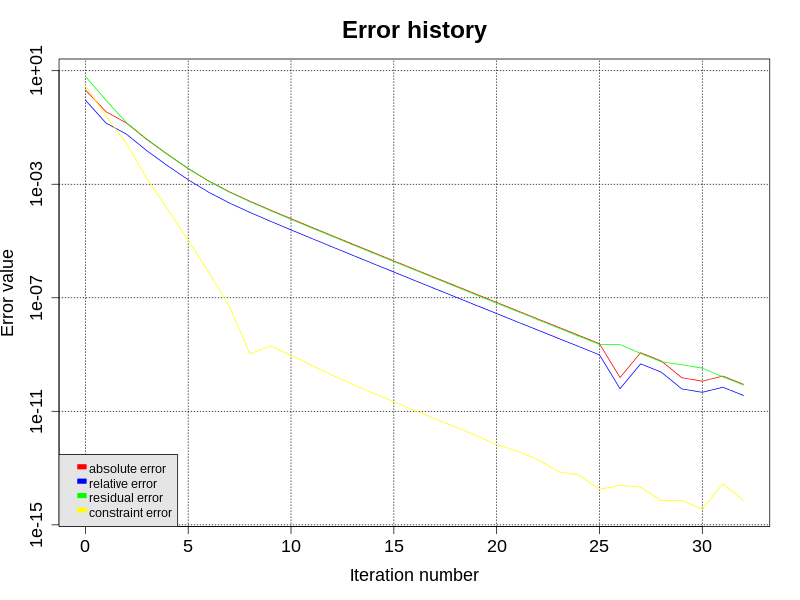
\includegraphics[width=10cm]{Figures/ErrorHistoryFORM.png}
               \end{center}
               \caption{Error history of the FORM algorithm.}
               \label{ErrorHist}
             \end{figure}